\documentclass[german]{spicker}
\usepackage{textcomp}
\usepackage{forest}

%\addbibresource{para.bib}

\title{Parallele Rechnerarchitekturen}
\subtitle{Sommersemester 2023}
\university{Fachhochschule Aachen}
\programme{Angewandte Mathematik und Informatik, M. Sc.}
\lecturer{Dr. Marcus Richter, Jochen Kreutz}

\author{Patrick Gustav Blaneck, Sven Bergmann}

\makeindex[intoc]
\makeindex[intoc, name=Beispiele,title=Beispiele]
\makeindex[intoc, name=Aufgaben,title=Aufgaben]


% Setup for SI units
\sisetup{
  per-mode=fraction,
  fraction-function=\tfrac
}
\DeclareSIUnit{\flops}{FLOPS}
\DeclareSIUnit{\cores}{cores}
\DeclareSIUnit{\cycle}{cycle}
\DeclareSIUnit{\cycles}{cycles}

% Forschungszentrum Jülich color
\definecolor{fzj}{rgb}{0, 0.24, 0.42}


\newenvironment{jsc}[2][\empty]{%
\ifx\empty#1
\index[Beispiele]{#2}%
\else
\index[Beispiele]{#1!#2}%
\fi
\label{jsc:#2}%
\begin{tcolorbox}[%
        colbacktitle=fzj!75!black,
        colback=fzj!5!white,%
        colframe=fzj!75!black,%
        base={#2},%
        label={%
                \ifx\empty#1
                {jsc:#2}%
                \else
                {jsc:#1:#2}
                \fi
            },
        % before title={%
        %         {\usekomafont{spickerboxtype}{Definition:}\hspace*{5mm}}
        %     },
        title={%
                \vphantom{Hy}%
                \usekomafont{spickerboxtitle}{{#2}}%
                \ifx\empty#1
                {}
                \else
                {
                    \hspace{2.5mm}\usekomafont{spickerboxsubtitle}{#1}
                }
                \fi
            },
        after title={%
                {\hfill\usekomafont{spickerboxtype}{Jülich Supercomputing Centre}}
            },
        % after title={
        %         {\usekomafont{spickerboxsubtitle}{
        %                     \ifx\empty#1
        %                     {\hfill}
        %                     \else
        %                     {\hfill #1}
        %                     \fi
        %                 }}
        %     },
    ]%
    }%
    {%

\end{tcolorbox}}


\newcommand{\aufgabe}[4][\empty]{
\ifx\empty#1
\index[Aufgaben]{#2}
\else
\index[Aufgaben]{#1!#2}
\fi
\label{Aufgabe:#2}
\begin{tcolorbox}[
        colbacktitle=red!75!black,
        colback=red!5!white,
        colframe=red!75!black,
        base={#2},
        label={
                \ifx\empty#1
                {Aufgabe:#2}%
                \else
                {Aufgabe:#1:#2}
                \fi
            },
        title={
                \vphantom{Hy}
                \usekomafont{spickerboxtitle}{{#2}}
                \ifx\empty#1
                {}
                \else
                {
                    \hspace{2.5mm}\usekomafont{spickerboxsubtitle}{#1}
                }
                \fi
            },
        after title={
                {\hfill\usekomafont{spickerboxtype}{Aufgabe}}
            },
    ]
    % \tcbsubtitle{Frage}
    % #3
    % \tcbsubtitle{Antwort}
    % #4
    \begin{tcolorbox}[enhanced, 
        title = Frage,
        attach boxed title to top right = {yshift=-2mm},
        boxed title style={
            colframe=red!75!black,
            colback=red!75!black
        },
        colback=red!5!white,
        colframe=red!75!black,
        % frame style={draw=none,fill=none},
        % watermark text = Frage,
        ]
        #3
    \end{tcolorbox}
    \tcblower
    \begin{tcolorbox}[enhanced, 
        title = Antwort,
        attach boxed title to top right = {yshift=-2mm},
        boxed title style={
            colframe=red!75!black,
            colback=red!75!black
        },
        colback=red!5!white,
        colframe=red!75!black,
        % frame style={draw=none,fill=none},
        % watermark text = Antwort,
        ]
        #4
    \end{tcolorbox}
\end{tcolorbox}
}

\begin{document}
\maketitle
\tableofcontents
\disclaimer

\section{Rechnerarchitekturen}\label{sec:rechnerarchitekturen}

\subsection{Einführung}\label{subsec:einfuehrung}

\begin{defi}{Struktur}
    Unter \emph{Struktur} versteht man die Art der Verknüpfung der verschiedenen Hardwarekomponenten eines Rechner miteinander.

    Sie ist in der Regel \emph{statisch}.
\end{defi}

\begin{defi}{Organisation}
    \emph{Organisation} steht für die zeitabhängigen Wechselwirkungen zwischen Komponenten und die Steuerung dieser Komponenten.

    Diese Wechselwirkungen können \emph{dynamisch} sein.
\end{defi}

\begin{defi}{Implementierung}
    \emph{Implementierung} bezeichnet die Ausgestaltung einzelner Bausteine.

    Sie gibt die \emph{Größe} eines Systems an.
\end{defi}

\begin{defi}{Leistung}
    \emph{Leistung} beschreibt das nach außen hin sichtbare Systemverhalten.

    Sie gibt die \emph{Geschwindigkeit} eines Systems an.
\end{defi}

\subsection{Von-Neumann-Rechner}\label{subsec:von-neumann-rechner}

\begin{defi}{Von-Neumann-Rechner}
    Der \emph{Von-Neumann-Rechner} besteht aus folgenden Werken:
    \begin{itemize}
        \item \emph{Eingabe- bzw. Ausgabewerk:}
        \begin{itemize}
            \item Schnittstelle zur Außenwelt
        \end{itemize}
        \item \emph{Leitwerk:}
        \begin{itemize}
            \item interpretiert Befehle
            \item steuert Abläufe
        \end{itemize}
        \item \emph{Haupt- bzw. Arbeitsspeicher:}
        \begin{itemize}
            \item Speicher für Daten und Befehle
        \end{itemize}
        \item \emph{Rechenwerk:}
        \begin{itemize}
            \item führt arithmetische und logische Operationen aus
        \end{itemize}
    \end{itemize}

    Die Struktur des Rechners ist unabhängig von der Aufgabe, die er lösen soll.
    Hardware und Software sind voneinander \emph{getrennt}.
\end{defi}

\begin{defi}[Von-Neumann-Rechner]{Struktur}

\end{defi}

\begin{defi}[Von-Neumann-Rechner]{Organisation}

\end{defi}

\begin{defi}[Von-Neumann-Rechner]{Arbeitsweise}
    \begin{itemize}
        \item Das Programm besteht aus einer \emph{Folge von Befehlen} (Instruktion),
        die nacheinander (sequentiell) ausgeführt werden.
        \item Von der Folge kann durch bedingte und unbedingte Sprungbefehle abgewichen werden, die die Programmfortsetzung an einer anderen Zelle bewirken.
        (Die bedingten Sprünge sind von gespeicherten Werten abhängig)
        \item Die Maschine benutzt Binärcodes, Zahlen werden dual dargestellt.
        Befehle und andere Daten müssen geeignet kodiert werden.
        Bitfolgen im Speicher sind nicht selbstidentifizierend.
    \end{itemize}
\end{defi}

\begin{defi}{Flaschenhals}
    \begin{itemize}
        \item Prozessor/Speicherschnittstelle ist kritisch für die Leistung des Gesamtsystems
        \item Daten werden vom Prozessor schneller verarbeitet als sie aus dem Speicher gelesen oder in den Speicher geschrieben werden können
        \item Durch Fortschritte in der Halbleitertechnik wurde die Diskrepanz zwischen Prozessorgeschwindigkeit und Speicherzugriffszeiten immer größer $\to$ \textbf{Flaschenhals (bottleneck)}
    \end{itemize}
\end{defi}

\subsection{Rechenleistung}\label{subsec:rechenleistung}

\begin{defi}{Leistung}
    Physikalisch: $P = \frac{W}{t}$, mit Leistung $P$, Arbeit $W$ und Zeit $t$
\end{defi}

\begin{defi}{Arbeit}
    Die Bearbeitung \ldots
    \begin{itemize}
        \item \ldots einer Instruktion (rechnerabhängig)
        \item \ldots einer Gleitkomma-Operation
        \item \ldots eines standardisierten Programms (Benchmark)
    \end{itemize}
\end{defi}

\begin{defi}[Leistungsmaß]{Clock-Rate}
    Die Taktfrequenz (engl.\ Clock-Rate) misst die Anzahl der Takte oder Zyklen, die von der CPU pro Sekunde durchgeführt werden in GHz (Gigahertz).
\end{defi}

\begin{defi}[Leistungsmaß]{FLOPS}
    Floating Point Operations Per Second
\end{defi}

\begin{bonus}{Top500}
    \begin{itemize}
        \item Erstellung der Liste der 500 schnellsten Rechner der Welt (2x pro Jahr)
        \item Leistungskriterium: Benchmark-Programme aus dem Gebiet der linearen Algebra (Linpack)
    \end{itemize}
    Aufbau:
    \begin{tabular}{|l|l|}
        Manufacturer      & Manufacturer or vendor                     \\
        Computer Type     & Indicated by manufacturer or vendor        \\
        Installation Site & Customer                                   \\
        Location          & Location and country                       \\
        Year              & Year of installation / last major update   \\
        Customer Segment  & Academic, Research, Industry, Vendor Class \\
        \# Processors     & Number of processors                       \\
        R max             & Maximal LINPACK performance achieved       \\
        R peak            & Theoretical peak performance               \\
        N max             & Problem size for achieving R max           \\
        N 1/2             & Problem size for achieving half of R max   \\
        N world           & Position within the TOP500 ranking         \\
    \end{tabular}
\end{bonus}

\begin{bonus}{Transistoren und Clock-Rate}
    Die Weiterentwicklung bei der Chipherstellung (Lithographie) führt zu feineren Strukturen auf einem Chip.

    Was passiert, wenn Leiterbahnen und Schaltelemente um einen Faktor $x$ schrumpfen ?
    \begin{itemize}
        \item Clock-Rate $f$ wächst um Faktor $x$ (Stromverbrauch, Abwärme $T \sim f^2$)
        \item Die Anzahl der Transistoren pro Fläche wächst mit $x^2$
        \item Die Rechenleistung des Chips wächst mit $x^4$ (aber der Zuwachs um $x^3$ beruht auf Architektur)
    \end{itemize}
\end{bonus}

\begin{defi}{Moore's Law}
    \label{defi:moores_law}
    \emph{Gordon Moore} (Mitbegründer von Intel) sagte 1965 voraus:
    \fbox{Die Anzahl der Transistoren auf einem Halbleiterchip verdoppelt sich ungefähr alle 18 Monate.}
    \[N = a\cdot 10^{\frac{1}{5}\cdot t}\]
\end{defi}

\begin{bonus}{Leistungslücke Prozessor-Memory}
    Aufgrund von~\nameref{defi:moores_law} wächst der \enquote{Performance Gap} (die Lesitungslücke) um ca.\ 50\% pro Jahr,
    da bisher die CPU-Performance um ca.\ 60\% pro Jahr und die DRAM-Performance nur um ca.\ 7\% pro Jahr gewachsen ist.
\end{bonus}

\section{Komplexität}\label{sec:komplexitaet}

\begin{defi}{Komplexität}
    Die \emph{Komplexität eines Algorithmus'} ist die Funktion $f(n)$, die den Aufwand für die benötigte Rechenzeit oder den benötigten Speicher in Abhängigkeit von der Problemgröße $n$ angibt.

    Die Komplexität ist abhängig von der Implementierung des Algorithmus'.

    Die \emph{Komplexität eines Problems} ist die minimale Komplexität aus einer Menge möglicher Algorithmen, die das Problem lösen.
\end{defi}

\begin{bonus}{Komplexitätsanalyse}
    Die \emph{Komplexitätsanalyse} untersucht z. B.:
    \begin{itemize}
        \item Wie viel Rechenzeit wird bei einer gegebenen Problemgröße $n$ benötigt?
        \item Wie ändert sich der Rechenzeitbedarf beim Anstieg von $n$?
        \item Ist der Rechenzeitbedarf noch realistisch und welcher Rechner kann das Problem in überschaubarer Zeit abarbeiten?
    \end{itemize}
\end{bonus}

\begin{defi}[Komplexität]{Problemgröße}
    Die \emph{Problemgröße} $n$ eines Programms bzw. Algorithmus' ist der Parameter, der den Aufwand für die benötigte Rechenzeit oder den benötigten Speicher bestimmt.
\end{defi}

\begin{defi}[Komplexität]{Rechenzeit}
    Die \emph{Rechenzeit} $T(n)$ eines Programms bzw. Algorithmus' ist die Anzahl der Rechenoperationen in Abhängigkeit von der Problemgröße $n$.

    Sie kann z. B. wie folgt berechnet werden:
    \[T(n) = a\cdot f(n) + t_b\]
    mit Rechenzeit $a$ für eine Rechen-, bzw. Gleitkomma-Operation und Rechenzeit $t_b$ für die Initialisierung und Beendigung des Algorithmus.
\end{defi}

\begin{defi}{Landau-Symbole}
    % TODO: https://de.wikipedia.org/wiki/Landau-Symbole (Quelle)
    \emph{Landau-Symbole} (auch \emph{O-Notation}) werden verwendet, um das asymptotische Verhalten von Funktionen und Folgen zu beschreiben.

    Die Komplexitätstheorie verwendet sie, um Probleme danach zu klassifizieren, wie \enquote{schwierig} oder aufwändig sie zu lösen sind.
    Zu \enquote{leichten} Problemen existiert ein Algorithmus, dessen Laufzeit sich durch ein Polynom beschränken lässt;
    als \enquote{schwer} gelten Probleme, für die man keinen Algorithmus gefunden hat, der weniger schnell als exponentiell wächst.

    % TODO: https://en.wikipedia.org/wiki/Big_O_notation (Quelle)
    Sei $f$ eine zu beschreibende reelle oder komplexe Funktion und $g$ eine reelle Vergleichsfunktion.

    $\mathcal{O}(g(n))$ bezeichnet eine Klasse von Funktionen, wobei
    \[ f(n) \in \mathcal{O}(g(n)) \]
    bedeutet, dass $f(n)$ höchstens so schnell wächst wie $g(n)$.
    Das widerum heißt, dass es zwei positive Konstanten $c$ und $n_0$ gibt, sodass
    \[ \forall n \geq n_0 : | f(n) | \leq c \cdot | g(n) | \]
\end{defi}

\begin{example}[Komplexitätsklassen]{Beschreibung}
    \begin{tabularx}{\linewidth}{llX}
        \toprule
        Klasse                  & Bezeichnung   & Beispiel                                                         \\
        \midrule
        $\mathcal{O}(1)$        & konstant      & Problem wird linear durchlaufen, unabhängig von Problemgröße     \\
        $\mathcal{O}(\log n)$   & logarithmisch & Binärsuche in einem sortierten Array                             \\
        $\mathcal{O}(n)$        & linear        & sequentielle Suche in einem unsortierten Array                   \\
        $\mathcal{O}(n \log n)$ & quasilinear   & \enquote{Divide-and-Conquer}-Algorithmen (Heap-Sort, Quick-Sort) \\
        $\mathcal{O}(n^2)$      & quadratisch   & einfache Sortieralgorithmen (Bubble-Sort, Selection-Sort)        \\
        $\mathcal{O}(n^c)$      & polynomiell   & Bestimmen der Determinante mithilfe von LU-Zerlegung             \\
        $\mathcal{O}(c^n)$      & exponentiell  & exaktes Lösen des Travelling-Salesman-Problems                   \\
        \bottomrule
    \end{tabularx}
\end{example}

\begin{example}[Komplexitätsklassen]{Visualisierung}
    \centering
    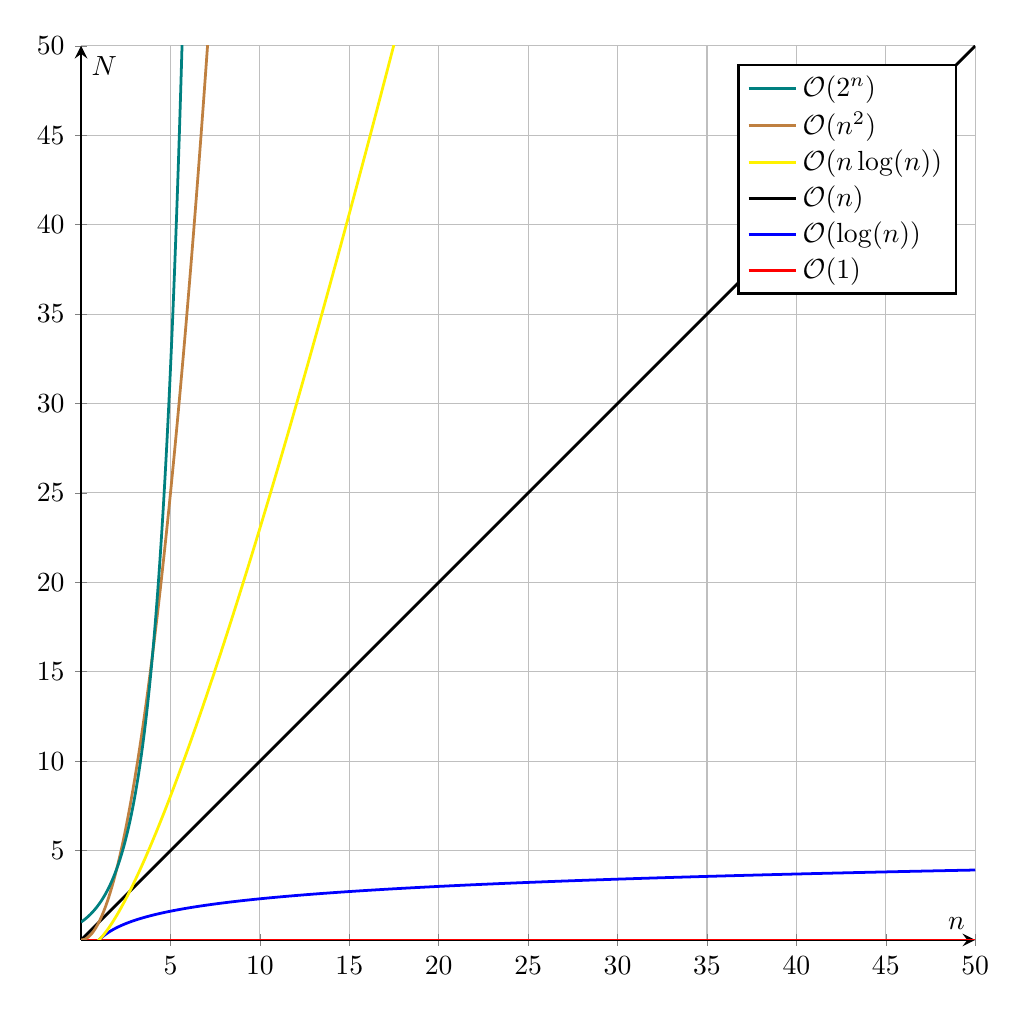
\begin{tikzpicture}[scale=1]
        \begin{axis}[
                width=15cm,
                unit vector ratio*=1 1,
                axis lines = middle,
                grid=major,
                ymin=0,
                ymax=50,
                xmin=0,
                xmax=50,
                xlabel = $n$,
                ylabel = $N$,
                xtick distance={5},
                ytick distance={5},
                disabledatascaling,
                cycle list name=color list,
                samples=250,
                solid,
                smooth,
                line width=1.0pt,
                no markers,
                legend cell align={left},
                reverse legend,
            ]

            \addplot +[domain=0:50]{0};         \addlegendentry{$\mathcal{O}(1)$};
            \addplot +[domain=0:50]{ln(x)};     \addlegendentry{$\mathcal{O}(\log(n))$};
                \addplot +[domain=0:50]{x};         \addlegendentry{$\mathcal{O}(n)$};
                \addplot +[domain=0:50]{x * ln(x)}; \addlegendentry{$\mathcal{O}(n \log(n))$};
            \addplot +[domain=0:50]{x^2};       \addlegendentry{$\mathcal{O}(n^2)$};
            \addplot +[domain=0:10]{2^x};        \addlegendentry{$\mathcal{O}(2^n)$};
        \end{axis}
    \end{tikzpicture}
\end{example}

\begin{example}[Komplexität]{Matrixmultiplikation}
    Problemgröße: $n$, ges.: $f(n)$ Anzahl der Rechen-Operationen in Abhängigkeit von der Matrix-Größe\\
    Notwendige Rechenzeit ist dann z.B.:
    \[T(n)=a\cdot f(n) + t_b\]
    mit $a$: Rechenzeit für eine Rechen- (Gleitkomma-) Operation,\\
    $b$: Rechenzeit für die Initialisierung und Beendigung des Algorithmus\\
    Formale Matrixmultiplikation:
    \[c_{i, j} = \sum\limits_{k=1}^{n}a_{i, k}\cdot b_{k, j}\]
    Bestimmung von $f(n)$: für jedes Element von $c$ sind $n$ Multiplikationen und $n-1$ Additionen durchzuführen.
    Also ergibt sich bei $n^2$ Elementen von $c$:
    \[f(n)=2\cdot n^3 - n^2\]

    TODO: Wording, Anschaulichkeit
\end{example}

\begin{bonus}{Master-Theorem}
    TODO
\end{bonus}

\begin{example}[Komplexität]{Strassen-Winograd}
    Effiziente Matrixmultiplikation:
    \begin{itemize}
        \item Matrizen werden in je vier Teilmatrizen der Größe $\frac{n}{2} \times \frac{n}{2}$ zerlegt:
              \begin{align*}
                  \begin{pmatrix}
                      A_{11} & A_{12} \\
                      A_{21} & A_{22}
                  \end{pmatrix}
                  \cdot
                  \begin{pmatrix}
                      B_{11} & B_{12} \\
                      B_{21} & B_{22}
                  \end{pmatrix}
                  =
                  \begin{pmatrix}
                      C_{11} & C_{12} \\
                      C_{21} & C_{22}
                  \end{pmatrix}
              \end{align*}
        \item Zusätzlich werden sieben neue Matrizen definiert:
              \begin{itemize}
                  \item $M_1 = (A_{12} - A_{22})\cdot(B_{21} + B_{22})$,
                  \item $M_2 = (A_{11} + A_{22})\cdot(B_{11} + B_{22})$,
                  \item $M_3 = (A_{11} - A_{21})\cdot(B_{11} + B_{12})$,
                  \item $M_4 = (A_{11} + A_{12})\cdot B_{22}$,
                  \item $M_5 = A_{11}\cdot(B_{21} - B_{22})$,
                  \item $M_6 = A_{22}\cdot(B_{21} - B_{11})$,
                  \item $M_7 = (A_{21} - A_{22})\cdot B_{11}$
              \end{itemize}
        \item Die vier Teilmatrizen der Ergebnismatrix ergeben sich damit wie folgt:
              \begin{itemize}
                  \item $C_{11} = M_1 + M_2 - M_4 + M_6$
                  \item $C_{12} = M_4 + M_5$
                  \item $C_{21} = M_6 + M_7$
                  \item $C_{22} = M_2 - M_3 + M_5 - M_7$
              \end{itemize}
    \end{itemize}
    Komplexität: $O(n^{\log_2 7})\approx O(n^2.807)$

\begin{defi}{Landau-Notation}
    Edmund Landau hat mit dem $O$-Symbol eine Notation geliefert,
    die den bestimmenden Term einer Funktion bezeichnet. \\
    $O(g(n))$ bezeichnet eine Klasse von Funktionen, wobei
    \[f(n) \in O(g(n))\]
    bedeutet, dass $f(n)$ höchstens so schnell wächst wie $g(n)$,
    das heißt, es gibt zwei positive Konstanten $c$ und $n_0$,
    für die gilt:
    \[|f(n)| \leq c \cdot |g(n)| \forall n \geq n_0\]
    (Definition hier nur für Funktionen über natürliche Zahlen)
\end{defi}

\begin{example}{Komplexitätsklassen}
    \begin{tabularx}{\textwidth}{|l|X|}
        \hline
        $O(1)$        & das Programm wird nur einmal linear durchlaufen, ohne von der Problemgröße abzuhängen (d.h. ohne Schleifen über $n$) $\to$ konstante Rechenzeit \\
        \hline
        $O(\log n)$   & z.B.\ bei Zerlegung von Problemen in Teilprobleme und Bearbeitung eines Teilproblems (binäre Suche)                                             \\
        \hline
        $O(n)$        & Algorithmen mit Schleifen $i = n_0 \ldots n$ (sequentielle Suche)                                                                               \\
        \hline
        $O(n \log n)$ & z.B.\ bei Zerlegung des Problems in Teilprobleme mit Bearbeitung aller Teilprobleme (Quicksort)                                                 \\
        \hline
        $O(n^2)$      & z.B.\ verschachtelte Schleifen (Paarweiser Vergleich)                                                                                           \\
        \hline
        $O(n^3)$      & z.B.\ dreifach verschachtelten Schleifen (Matrixmultiplikation)                                                                                 \\
        \hline
        $O(2n)$       & z.B.\ Suche in allen Kombinationen, Paaren oder Teilmengen                                                                                      \\
        \hline
    \end{tabularx}
\end{example}




\section{Parallelverarbeitung}\label{sec:parallelverarbeitung}

\begin{defi}{Parallelverarbeitung}
    Durch Aufteilung einer Aufgabe in Teilaufgaben,
    die gleichzeitig bearbeitet werden können,
    soll eine Leistungssteigerung erzielt werden.\\
    Man unterscheidet:
    \begin{itemize}
        \item \underline{Sequentielle Verarbeitung:} nacheinander ausführen der Teilaufgaben
        \item \underline{Parallele Verarbeitung:} es gibt Zeitabschnitte in der Verarbeitung, in der Teilaufgaben gleichzeitig bearbeitet werden
    \end{itemize}
    \underline{Voraussetzungen:}
    \begin{enumerate}
        \item Aufteilungsmöglichkeit existiert und wird erkannt
        \item mehrere Bearbeiter stehen zur Verfügung
        \item gleichzeitig $\to$ möglichst unabhängig
    \end{enumerate}
\end{defi}

\begin{defi}[Parallelverarbeitung]{Domain Decomposition}
    Statische oder dynamische Aufteilung eines Datengebiets in Bereiche gleicher Prozessorarbeit.
    Alle Gebiete werden mit demselben Programmteil parallel verarbeitet.
    \begin{itemize}[$\to$]
        \item Kommunikation erfordert \enquote{enggekoppelte} Prozessoren
        \item geeignet für homogene Plattformen
        \item am häufigsten verwendet in HPC
    \end{itemize}
\end{defi}

\begin{defi}[Parallelverarbeitung]{Functional Decomposition}
    Unterschiedliche Programmteile, Unterprogramme,
    Module werden auf Prozessoren verteilt und parallel bearbeitet.
    \begin{itemize}[$\to$]
        \item verschiedene Rechnerarchitekturen für unterschiedliche Programmteile einsetzbar
        \item aufwändiger zu Implementieren
    \end{itemize}
\end{defi}

\begin{bonus}{Modular Supercomputing Architecture}
    
\end{bonus}

\begin{defi}{Speedup}
    \ldots ist ein Maß für die Bewertung der Verarbeitung eines einzelnen Auftrages (Passagiers).
\end{defi}

\begin{defi}{Durchsatz}
    \ldots ist ein Maß für die Bewertung der Verarbeitung einer gesamten Arbeitslast
    (mit welchem Flugzeug kann eine Fluggesellschaft mehr Personen befördern ?).
\end{defi}

\begin{defi}{Amdahl's Law}
    \begin{align*}
        \text{Speedup }S(p)=
        \frac{\text{Laufzeit (sequentiell)}}{\text{Laufzeit (parallel)}} =
        \frac{T_s}{T_S \cdot f + (1-f) \cdot \frac{T_s}{p}}
    \end{align*}
    mit:
    \begin{itemize}
        \item $p:$ Anzahl der parallelen Bearbeitungselemente (Prozessoren)
        \item $T_s:$ Laufzeit für die sequentielle Bearbeitung der gesamten Aufgabe
        \item $f:$ Anteil der Laufzeit, die für Teile verbraucht wird, die nicht parallel ablaufen können
    \end{itemize}
    für:
    \begin{itemize}
        \item $p\to\infty: S(\infty) = \frac{1}{f} \text{, oder} T(\infty) = f \cdot T_s$
        \item $f\to 0: S(p) = p \text{, oder} T(p) = \frac{T_s}{p}$
    \end{itemize}
\end{defi}

\begin{defi}{Effizienz}
    Effizienz definiert das Verhältnis von Speedup und eingesetzter Prozessoranzahl.
    Sie drückt aus, welcher Anteil der Prozessorleistung nutzbar ist.
    \begin{align*}
        E(p) = \frac{S(p)}{p} =
        \frac{T(\text{sequentiell})}{p\cdot T(\text{parallel})},
        0<E(p)\leq 1
    \end{align*}
\end{defi}

\begin{example}[Speedup]{Skalarprodukt}
    Paralleler Algorithmus:
    \begin{enumerate}
        \item Aufteilen in $p$ Teilvektoren der Länge $\frac{n}{p}$
        \item jeder Prozessor berechnet das Skalarprodukt des Teilvektors $T_* (p) = \left(2 \cdot \frac{n}{p} - 1\right) \cdot t_\text{flop}$
        \item die Ergebnisse werden zu Prozessor 1 übertragen $T_t (p) = (p - 1) \cdot (t_\text{startup} + t_\text{word})$
        \item und Addition der Teilergebnisse (reduzieren) $T_+ (p) = (p - 1) \cdot t_\text{flop}$
    \end{enumerate}
    für $p=2^d$:
    \begin{align*}
        S(p) = \frac{T(\text{seq})}{T(p)} = \ldots =
        \frac{p}{\frac{p(\frac{2n}{p} + d-1)}{2n-1} + \frac{p\cdot d\cdot (t_\text{startup} + t_\text{word})}{(2n - 1)t_\text{flop}}}
    \end{align*}
    bei $n\gg p$:
    \begin{align*}
        \approx\frac{p}{
        \underbrace{1 + p\cdot \log_2 p}_{\text{Algorithmus}} \cdot
        \underbrace{\frac{1}{2n}}_{\text{Problemgröße}} \cdot
        \underbrace{\frac{t_\text{startup}}{t_\text{flop}}}_{\text{Hardware}}}
    \end{align*}
\end{example}

\begin{example}[Effizienz]{Skalarprodukt}
    \begin{align*}
        E(p)\approx\frac{1}{1 + p\cdot\log_2 p\cdot \frac{1}{2n} \cdot \frac{t_\text{startup}}{t_\text{flop}}}
    \end{align*}
    Die Effizienz \emph{steigt} mit wachsender Problemgröße $n$ (bei $p$ fest) und
    \emph{sinkt} bei größerer Prozessoranzahl $p$ (mit $n$ fest)
\end{example}

\begin{defi}{Skalierbarkeit}
    Eine Rechnerarchitektur bzw.\ ein Programm ist skalierbar,
    wenn die Effizienz der Programmbearbeitung bei wachsender Prozessorzahl gleich bleibt.
\end{defi}

\begin{defi}{Pipelining}
    Henry Ford hat 1913 mit Produktionsbeginn der \enquote{Tin Lizzy} als erster das Fließband in die industrielle Fabrikation eingeführt.
    Prinzip: Ein komplexer Vorgang wird in eine Sequenz von einfacheren Teilaufgaben zerlegt. \\
    Vorteile:
    \begin{itemize}
        \item Höherer Durchsatz ($\frac{\text{Lizzy}}{h}$)
        \item Vereinfachung (und damit auch eine schnellere Bearbeitung) der Teilaufgaben (CISC $\to$ RISC)
    \end{itemize}
\end{defi}
\section{Einzelprozessorsysteme}\label{sec:einzelprozessorsysteme}

\begin{defi}{Überlappte Verarbeitung}
    Erstes Ziel war die überlappte Verarbeitung von langsamen und schnellen Hardware-Komponenten. 
    (Verstecken der langsamen Funktionseinheiten)
\end{defi}

\begin{defi}{Überlappter I/O}
    Während des langsamen I/O kann nun gleichzeitig die \enquote{wertvolle} Ressource CPU genutzt werden.
\end{defi}

\subsection{Cache}\label{subsec:cache}

\begin{defi}{Cache}
    \ldots ist ein schneller Speicher mit verhältnismäßig kleiner Speicherkapazität, 
    der zwischen der Zentraleinheit (CPU) und dem Arbeitsspeicher positioniert ist.
\end{defi}

\begin{defi}{Direct Mapped Cache}
    Feste Abbildung der Hauptspeicher-Adressen auf die Cache-Adressen
    \begin{itemize}[$\to$]
        \item Kein assoziativer Speicher nötig
        \item Keine Verdrängungsstrategien nötig
    \end{itemize}
\end{defi}

\begin{defi}{N-way Set Associative Cache}
    N-fache Mengenassoziativität: $N$ Einträge pro Cache-Index \\
    \quad $\to$ $N$ Caches mit direkter Abbildung, die parallel operieren
    ($N$ liegt meist zwischen 2 und 4)\\
    Beispiel: zweifach mengenassoziativer Cache
    \begin{itemize}
        \item Der Cache-Index bestimmt eine \enquote{Menge} von Blöcken im Cache
        \item Die beiden Tags werden parallel verglichen.
        \item Die Daten werden aufgrund des Tagvergleichs selektiert.
    \end{itemize}
\end{defi}

\begin{defi}{Fully Associative Cache}
    
\end{defi}

\begin{defi}{Ersetzungsstrategie}
    \begin{itemize}
        \item Trivial für Direct Mapped Cache
        \item Bei Set Associative oder Fully Associative:
              \begin{itemize}
                  \item Random
                  \item LRU (Least Recently Used) bzw. FIFO
              \end{itemize}
    \end{itemize}
    Zurückschreiben von Daten:
    \begin{itemize}
        \item \underline{Write through:} Die Information wird sowohl in den Cache als auch ins
              Memory zurückgeschrieben.
        \item \underline{Write back:} Die Information wird nur in den Cache geschrieben. Die
              veränderte Zeile wird erst dann ins Memory geschrieben, wenn die
              Cache-Zeile mit Daten aus anderen Hauptspeicheradressen
              überschrieben werden soll.
              \begin{itemize}
                  \item \underline{Vorteil:} Mehrfaches Ändern eines Wertes wird nur im Cache durchgeführt.
                  \item \underline{Nachteil:} Ein Read-Miss kann zu einem Schreiben ins Memory führen.
              \end{itemize}
    \end{itemize}
\end{defi}

\begin{bonus}[Cache]{IBM Power 4}
    
\end{bonus}

\begin{bonus}[Cache]{Intel Itanium}
    
\end{bonus}

\begin{defi}{Cache Miss}
    Ist keine Kopie der Hauptspeicherzelle a im Cache abgelegt, so 
    \begin{itemize}
        \item greift die CPU auf den Arbeitsspeicher zu,
        \item lädt das Datum in den Cache und
        \item lädt das Datum gleichzeitig in die CPU.
    \end{itemize}
\end{defi}

\begin{defi}{Reduzierung der Cache Miss Rate}
    \begin{itemize}
        \item \underline{Cold start miss:} Tritt auf beim ersten Zugriff auf einen Block nach dem Start des Programms oder dem Task-Wechsel (auch bei unendlich großem Cache)
        \item \underline{Capacity miss:} Tritt auf, wenn der Cache nicht alle Blocks speichern kann, die bei der Ausführung durch die CPU benötigt werden (nur bei fully associative Cache)
        \item \underline{Conflict miss:} Tritt auf, wenn ein Block ersetzt werden muß, der anschließend wieder benötigt wird (bei N-way associative Cache)
        \item \underline{Coherence miss:} bei Mehrprozessorsystemen → wird später erklärt
    \end{itemize}
\end{defi}

\begin{defi}[Reduzierung der Cache Miss Rate]{Programmierstrategien}
    Verbessern der Speicherlokalität durch
    \begin{itemize}[\ldots]
        \item Datenstrukturierung
        \item Ändern der Indexierung
        \item Schleifenfusion
        \item Bildung von Teilblöcken
    \end{itemize}
\end{defi}

\begin{defi}{Table-Look-Aside Buffer}
    Bei Rechnern mit virtueller Speicherverwaltung arbeitet der Prozessor mit virtuellen Adressen, 
    die durch den TLB in reale Adressen umgesetzt werden.
\end{defi}

\subsection{Entwicklungslinien der Prozessoren}\label{subsec:entwicklungslinien-der-prozessoren}

\begin{defi}{Complex Instruction Set Computer (CISC)}
    Befehls-Code ist Index auf Zeiger-Array für Mikroprogramm,
    die Hardware führt die Sequenz der Mikrobefehle aus.
\end{defi}

\begin{defi}{Reduced Instruction Set Computer (RISC)}
    Der Compiler erzeugt direkt \enquote{Mikrobefehle}. 
    Es muss zwar mehr Code erzeugt werden, 
    aber die Hardware wird einfacher und damit auch schneller.
\end{defi}

\begin{defi}{Very Long Instruction Word (VLIW)}
\end{defi}

\begin{defi}{Explicitly Parallel Instruction Computing (EPIC)}
    Von HP und Intel wurde 1998/99 die Prozessorarchitektur EPIC entworfen 
    und mit dem Intel Itanium ein erster Prozessor realisiert. 
    Die Intel-Version der Architektur wird IA-64 (64 bit) genannt.
    
    EPIC ist die moderne Weiterentwicklung des Konzepts des VLIW.
    
    Hierbei versucht der Compiler, 
    möglichst viele voneinander unabhängige Instruktionen in einer Sequenz zusammenzustellen. 
    Er kann dabei durch Umstellen der Befehle die Reihenfolge innerhalb der Sequenz verändern. 
    Dies darf aber nicht zu anderen Ergebnissen führen!
    
    Eine solche Sequenz nennt Intel ein “bundle”.
\end{defi}

\section{Pipelining}

\begin{defi}{Pipelining}
    Durch Aufteilen einer Instruktion in Teile, 
    die in separaten Funktionseinheiten bearbeitet werden können, 
    ist eine überlappte (pseudo-parallele) Verarbeitung der Instruktionen möglich.
\end{defi}

\begin{defi}[Pipelining]{Funktionseinheiten}
    Eine 5-stufige Pipeline (z.B. MIPS-Prozessor) wird aus folgenden Funktionseinheiten gebildet:
    \begin{center}
        \begin{tabular}{ll}
            IF:  & Instruction Fetch  \\
            ID:  & Instruction Decode \\
            EX:  & Execution          \\
            MEM: & Memory Access      \\
            WB:  & Write Back         \\
        \end{tabular}
    \end{center}
\end{defi}

\begin{defi}[Pipelining]{Latenz}
    Wie groß ist die Laufzeit für eine einzelne Instruktion?
    \[T_\text{instr} = T_\text{IF} + T_\text{ID} + T_\text{EX} + T_\text{MEM} + T_{WB}\]
\end{defi}

\begin{defi}[Pipelining]{Durchsatz}
    Wie oft pro Zeiteinheit wird eine Instruktion fertig ?
    \[X = \frac{1}{\max(T_\text{IF}, T_\text{ID}, T_\text{EX}, T_\text{MEM}, T_{WB})}\]
\end{defi}

\begin{defi}{Superskalarität}
    
\end{defi}

\begin{defi}{Instruction Level Parallelism (ILP)}\label{defi:ilp}
    \emph{Instruction Level Parallelism (ILP)} oder Parallelität auf Anweisungsebene ist die parallele oder gleichzeitige Ausführung einer Folge von Anweisungen in einem Computerprogramm. 
    Genauer gesagt bezieht sich ILP auf die durchschnittliche Anzahl der Anweisungen, die pro Schritt dieser parallelen Ausführung ausgeführt werden.
\end{defi}

\begin{defi}{Hazards}
    \begin{itemize}
        \item \underline{Structural hazards:}
              Die HW kann nicht eine bestimmte Aufeinanderfolge von Instruktionen ausführen.
        \item \underline{Data hazards:}
              Instruktionen hängen vom Ergebnis vorheriger Schritte ab, 
              die noch nicht die Pipeline verlassen haben.
        \item \underline{Control hazards:}
              Zwischen dem \enquote{fetch} von Instruktionen und dem Ändern des Kontrollflusses (branch) entstehen Verzögerungen.
    \end{itemize}
\end{defi}

\begin{defi}{Schleifenparallelisierung}
    Ziel ist es, 
    den Schleifenkörper ohne stottern durch die vorhandenen Funktionsinheiten zu schicken.
    Dazu sind Abhängigkeiten zwischen den Anweisungen zu finden und, 
    wenn möglich, zu beseitigen.
\end{defi}

\begin{defi}{Abhängigkeitsgraph}
    
\end{defi}

\begin{defi}{Predication}
    Mit der Predication-Methode können bestimmte Control Hazards (branches) aufgelöst werden, 
    z. B. 'If-then-else'-Konstrukte
\end{defi}

\begin{defi}{Data Speculation}
    Durch Umstellen der Befehlsreihenfolge (z. B. Laden von Daten) kann Parallelität erhöht werden.
\end{defi}

\begin{defi}{Control Speculation}
    Durch Umstellen der Befehlsreihenfolge (z. B. Ausführung von Operationen) kann Parallelität erhöht werden.
\end{defi}

\begin{defi}{Attached-Processor-Systeme}
    Eine zusätzliche Einheit, 
    die in einer Multiprozessor-Umgebung an die primäre CPU angeschlossen ist. 
    Sie arbeitet als Erweiterung der primären CPU und 
    nutzt die Systemsoftware und Peripheriegeräte gemeinsam.
\end{defi}
\section{Mehrprozessorsysteme}

\begin{defi}{Flynn'sche Klassifikation}
    Von Flynn wurde 1972 eine sehr grobe aber heute noch häufig genutzte Unterscheidung von Parallelrechnern eingeführt.
    Sie orientiert sich an der Anzahl der gleichzeitig vorhandenen Instruktions- und Datenströme.
    
    Parallelrechner:
    
    \begin{center}
        \begin{tabular}{ll}
            SISD & Single Instruction Single Data (Von Neumann-Rechner $\to$ kein paralleles System) \\
            SIMD & Single Instruction Multiple Data                                                  \\
            MISD & Multiple Instruction Single Data $\to$ \textbf{irrelevant!}                       \\
            MIMD & Multiple Instruction Multiple Data 
        \end{tabular}
    \end{center}
\end{defi}

\begin{bonus}[Flynn'sche Klassifikation]{Erweiterungen}
    \begin{itemize}
        \item \emph{SIMD} Single Instruction Multiple Data
              \begin{itemize}
                  \item Vektor-Prozessoren (auch Mischformen mit MIMD vorhanden!)
                  \item Array-Prozessoren
              \end{itemize}
        \item \emph{MIMD} Multiple Instruction Multiple Data
              \begin{itemize}
                  \item Speichergekoppelte Multiprozessoren
                        \begin{itemize}
                            \item Unified Memory Architecture (UMA)
                            \item Non-Uniform Memory Access (NUMA)
                        \end{itemize}
                  \item Nachrichtengekoppelte Multiprozessoren
                        \begin{itemize}
                            \item Massively Parallel Processing (MPP)
                            \item Cluster Of Workstations (COW)
                        \end{itemize}
              \end{itemize}
    \end{itemize}
\end{bonus}

\subsection{Speichergekoppelte Systeme}

\begin{defi}{Speichergekoppelte Systeme}
    Bei speichergekoppelten Multiprozessoren arbeiten alle Prozessoren in einem einheitlichen Adressraum.
    
    Je nach physiklischer Speicherorganisation unterscheidet man:
    \begin{itemize}
        \item Symmetrische Multiprozessoren (SMP, symmetric multiprocessor),
              bei denen gleichartige Prozessoren über ein Verbindungsnetzwerk mit einem gemeinsamen Speicher verbunden sind
        \item Distributed-Shared-Memory Systeme,
              bei denen zwar ein einheitlicher Adressraum existiert, 
              aber die Speicher physikalisch auf einzelnen Verarbeitungsknoten verteilt sind
    \end{itemize}
    
    \emph{Bemerkungen:}
    \begin{itemize}
        \item Speichergekoppelte Multiprozessoren gelten als einfacher programmierbar gegenüber nachrichtengekoppelten Multiprozessoren
        \item Nutzbare Parallelität reicht von der Programmebene bis zur Blockebene
        \item Autoparallelisierende Compiler nutzen insbesondere die Parallelisierung der Schleifenebene (einzelne Iterationen nebenläufig abarbeitbar)
    \end{itemize}
\end{defi}

\begin{defi}{Uniform Memory Access}
    Kapitel 5 Seite 8
\end{defi}

\begin{defi}{Non-Uniform Memory Access}
    Kapitel 5 Seite 9
\end{defi}

\begin{defi}{Nachrichtengekoppelte Systeme}
    Kapitel 5 Seite 10
\end{defi}

\subsection{Verbindungsnetzwerke}

\begin{defi}{Verbindungsnetzwerk}
    Ein Verbindungsnetzwerk ermöglicht den Datenaustausch (und die Verteilung des Programms) zwischen den Prozessoren.
    
    Um einen hohen Datentransfer zu erhalten, 
    wird eine große Anzahl von Drähten benötigt!
    
    Ein VN gleicht einer Straße:
    \begin{itemize}
        \item Link = Straße
        \item Switch = Kreuzung
        \item Distance/Hops = Anzahl der zurückgelegten Straßenblöcke
        \item Routing algorithm = Reiseplan
    \end{itemize}
    
\end{defi}

\begin{defi}[Verbindungsnetzwerk]{Latenz}
    Zeit für den Transfer zwischen den Knoten
\end{defi}

\begin{defi}[Verbindungsnetzwerk]{Bandbreite}
    \[\frac{\text{transferierte Daten}}{\text{Zeit}}\]
    Bandbeite eines Link: $\text{bw} = w \cdot \frac{1}{t}\frac{\text{bit}}{\text{sec}}$
    mit $w$: Anzahl der Drähte
\end{defi}

\begin{defi}[Verbindungsnetzwerk]{Durchmesser}
    maximale Distanz zwischen zwei beliebigen Prozessoren
\end{defi}

\begin{defi}[Verbindungsnetzwerk]{Topologie}
    Wie sind die Nachbarknoten angeordnet und erreichbar?
\end{defi}

\subsubsection{Statische Verbindungsnetzwerke}

\begin{defi}{Lineare Anordnung}
    \begin{center}
        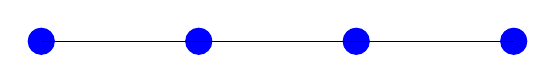
\begin{tikzpicture}
            \node[circle, draw=blue, fill=blue] (d0) at (0, 0) {};
            \node[circle, draw=blue, fill=blue] (d1) at (2, 0) {};
            \node[circle, draw=blue, fill=blue] (d2) at (4, 0) {};
            \node[circle, draw=blue, fill=blue] (d3) at (6, 0) {};
            \draw (d0.center) to[out=0, in=180] (d1.center);
            \draw (d1.center) to[out=0, in=180] (d2.center);
            \draw (d2.center) to[out=0, in=180] (d3.center);
        \end{tikzpicture}
        \\
        Diameter = $N-1$
    \end{center}
\end{defi}

\begin{defi}{Torus oder Ring}
    \begin{center}
        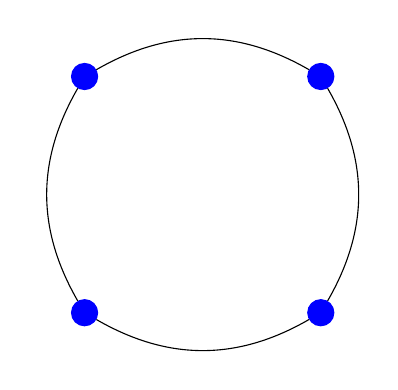
\begin{tikzpicture}
            \node[circle, draw=blue, fill=blue] (d0) at (3.5, 0.5) {};
            \node[circle, draw=blue, fill=blue] (d1) at (3.5, 3.5) {};
            \node[circle, draw=blue, fill=blue] (d2) at (0.5, 3.5) {};
            \node[circle, draw=blue, fill=blue] (d3) at (0.5, 0.5) {};
            \draw (d0) to[bend right] node[left]{}(d1);
            \draw (d1) to[bend right] node[left]{}(d2);
            \draw (d2) to[bend right] node[left]{}(d3);
            \draw (d3) to[bend right] node[left]{}(d0);
        \end{tikzpicture}
        \\
        Diameter = $\frac{N}{2}$
    \end{center}
\end{defi}

\begin{defi}{Torus}
    2D-Torus:
    \begin{center}
        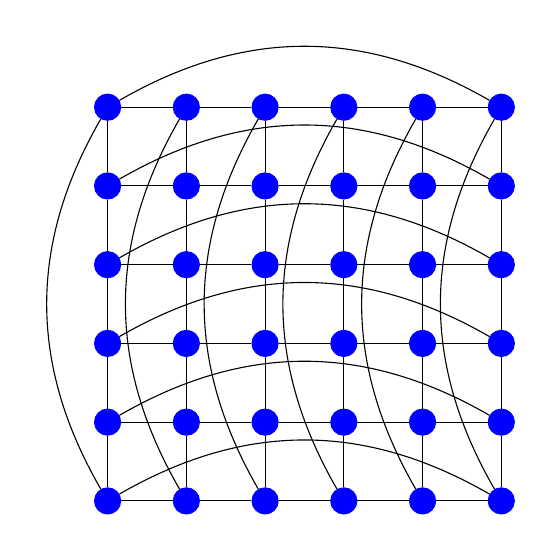
\begin{tikzpicture}[circlestyle/.style={circle, draw=blue, fill=blue}]
            \foreach \x in {0, ..., 5}
            \foreach \y in {0, ..., 5}
            \node[circlestyle] (\x\y) at (\x, \y) {};
            
            \foreach \x in {0,...,5}
            \foreach \y [count=\yi] in {0,...,4}
            \draw (\x\y)--(\x\yi) (\y\x)--(\yi\x); 
            
            \draw (00) to[bend left] node[left]{}(05);
            \draw (10) to[bend left] node[left]{}(15);
            \draw (20) to[bend left] node[left]{}(25);
            \draw (30) to[bend left] node[left]{}(35);
            \draw (40) to[bend left] node[left]{}(45);
            \draw (50) to[bend left] node[left]{}(55);
            
            \draw (00) to[bend left] node[left]{}(50);
            \draw (01) to[bend left] node[left]{}(51);
            \draw (02) to[bend left] node[left]{}(52);
            \draw (03) to[bend left] node[left]{}(53);
            \draw (04) to[bend left] node[left]{}(54);
            \draw (05) to[bend left] node[left]{}(55);
        \end{tikzpicture}
    \end{center}
\end{defi}

\begin{defi}{Gitter}
    2D-Gitter:\\
    Diameter = $2\cdot\left(\sqrt{N} - 1\right)$
    \begin{center}
        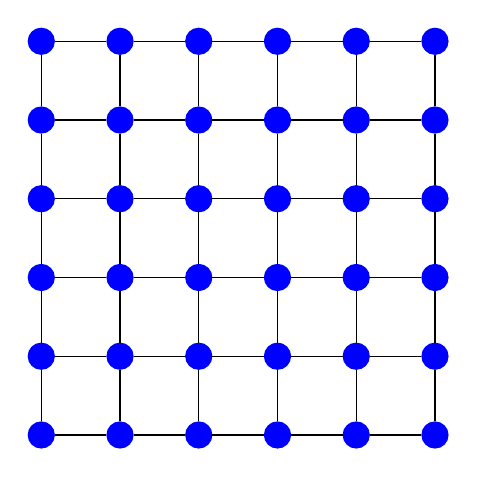
\begin{tikzpicture}[circlestyle/.style={circle, draw=blue, fill=blue}]
            \foreach \x in {0, ..., 5}
            \foreach \y in {0, ..., 5}
            \node[circlestyle] (\x\y) at (\x, \y) {};
            
            \foreach \x in {0,...,5}
            \foreach \y [count=\yi] in {0,...,4}
            \draw (\x\y)--(\x\yi) (\y\x)--(\yi\x); 
        \end{tikzpicture}
    \end{center}
\end{defi}

\begin{defi}{Hypercube}
    \begin{itemize}
        \item Anzahl der Knoten: $N = 2d$
        \item Diameter: $d = \log_2 N$
        \item Greycode Adressierung: Jeder Knoten verbunden mit $d$ anderen Knoten unterscheidet sich durch \emph{ein Bit} in der Adresse
        \item Beispiele: Intel iPSC und NCUBE
        \item 0d:
              
\begin{tikzpicture}[circlestyle/.style={circle, draw=blue, fill=blue}]
                  \node[circlestyle] (A) at (0,0) {};
              \end{tikzpicture}
        \item 1d:
              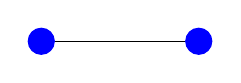
\begin{tikzpicture}[circlestyle/.style={circle, draw=blue, fill=blue}]
                  \node[circlestyle] (A) at (0,0) {};
                  \node[circlestyle] (B) at (2,0) {};
                  \draw (A) to[] node[left]{}(B);
              \end{tikzpicture}
        \item 2d:
              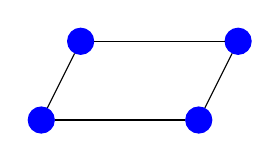
\begin{tikzpicture}[circlestyle/.style={circle, draw=blue, fill=blue}]
                  \node[circlestyle] (A) at (0,0) {};
                  \node[circlestyle] (B) at (2,0) {};
                  \draw (A) to[] node[left]{}(B);
                  
                  \node[circlestyle] (C) at (0.5, 1) {};
                  \node[circlestyle] (D) at (2.5, 1) {};
                  \draw (C) to[] node[left]{}(D);
                  
                  \draw (A) to[] node[left]{}(C);
                  \draw (B) to[] node[left]{}(D);
              \end{tikzpicture}
        \item 4d: TODO!
    \end{itemize}
    TODO: tikzpicture
\end{defi}

\begin{defi}{Baum}
    Diameter = $\log_2 N$
    \begin{itemize}
        \item Planares Layout:
              TODO: tikzpicture
        \item Fetter Baum: (mehr Verbindungen erhöhen das Datenvolumen)
    \end{itemize}
\end{defi}

\begin{bonus}{Übersicht statischer Verbindungsnetzwerke}
    \begin{tabularx}{\textwidth}{|l|X|X|X|}
        \hline
        Topologie          & Anzahl der Verbindungskanäle pro Knoten & Maximale Entfernung (Diameter) & Gesamtanzahl der Verbindungskanäle \\
        \hline
        Ring               & 2                                       & $\frac{N}{2}$                  & $N-1$                              \\
        \hline
        Baum               & 3                                       & $2\cdot (\log_2 N - 1)$        & $N-1$                              \\
        \hline
        2D - Gitter        & 4                                       & $2\cdot \sqrt{N}$              & $2\cdot N$                         \\
        \hline
        3D - Gitter        & 6                                       & $3\cdot \sqrt[3]{N}$           & $3\cdot N$                         \\
        \hline
        Hexagon. Gitter    & 6                                       & $3\cdot \sqrt[3]{N}$           & $3\cdot N$                         \\ 
        \hline
        Hypercube          & $\log_2 N$                              & $\log_2 N$                     & $N \log_2 \frac{N}{2}$             \\
        \hline
        Vollst. Vernetzung & $N - 1$                                 & 1                              & $N \cdot \frac{N-1}{2}$            \\
        \hline
    \end{tabularx}
\end{bonus}

\subsubsection{Dynamische Verbindungsnetzwerke}

\begin{defi}{Bus}
    \begin{itemize}
        \item Durch die wahlweise Zuschaltung einzelner Verarbeitungsknoten zum Datentransfer an einen Bus ist das Bussystem eine typische dynamische Verbindungseinrichtung
        \item Der Bus bildet die Engstelle im busgekoppelten Multiprozessorsystem,
              so dass auch Doppelbusse oder allgemein Mehrfachbusse eingesetzt werden
        \item Bussysteme und auch Mehrbussysteme werden für Systeme mit höchstens 30 Prozessoren eingesetzt,
              um Zugiffskonflikte in Grenzen zu halten
    \end{itemize}
\end{defi}

\begin{defi}{Crossbar}
    \begin{itemize}
        \item $M \times M$ Matrix
        \item einfaches Weiterleiten an mehrere Ausgänge
        \item komplexe Steuerung
        \item Verdrahtungsaufwand
        \item Pufferung bei Blockierungen
        \item Diameter = 1, d. h. beliebige Verbindungen können unter Einsatz jeweils nur einer Schaltzelle realisiert werden
    \end{itemize}
\end{defi}

\begin{defi}{Zellenbasierte Systeme}
    Zellen mit 2 Eingängen und 2 Ausgägen bilden die Basis für solche Systeme.
    \begin{itemize}
        \item 2 Bit $\to$ 4 Schaltzustände
        \item gerade Zellen
        \item kreuzende Zellen
        \item Eingänge mit mehreren Ausgängen verbunden (seltener genutzt)
    \end{itemize}
\end{defi}

\begin{defi}{Einstufige Netzwerke}
    Eine Spalte von Schaltzellen wird durch Rückkopplung der Ausgänge auf die Eingänge Verbunden. 
    Die Zellen werden mehrfach durchlaufen.
\end{defi}

\begin{defi}{Mehrstufige Netzwerke}
    Mehrere Spalten von Schaltzellen, auch mit Rückführungen, 
    sind fest miteinander verbunden.
\end{defi}

\begin{defi}{Omega-Netzwerk}
    TODO: Including images does not work!
    % \begin{figure}[H]
    %     \centering
    %     \includegraphics{graphics/OmegaNetwork.jpg}
    %     \caption{By Bjmyers17, CC BY-SA 3.0, https://commons.wikimedia.org/w/index.php?curid=75639225}
    % \end{figure}
\end{defi}

\begin{defi}{Benes-Netzwerk}
    TODO: Including images does not work!
    % \begin{figure}[H]
    %     \centering
    %     \includegraphics{graphics/Benesnetwork.png}
    %     \caption{By Piggly - Own work, Public Domain, https://commons.wikimedia.org/w/index.php?curid=2988080}
    % \end{figure}
\end{defi}

\subsubsection{Cluster-Interconnects}

\begin{defi}{Cluster-Interconnect}
    
\end{defi}

\begin{defi}{Infiniband}
    \begin{itemize}
        \item \ldots ist eine Architektur für Hochgeschwindigkeitsverbindungen zwischen Rechnern und externen Speicherservern.
        \item \ldots wurde unter Führung von Intel entwickelt, später Mellanox, jetzt Nvidia.
        \item \ldots eignet sich auch als Verbindungsnetzwerk von Rechen-Clustern.
    \end{itemize}
    aktuell: Infiniband EDR / HDR mit bis zu 200 Gbit/s
\end{defi}

\begin{defi}{Gigabit Ethernet}
    \begin{itemize}
        \item \ldots wird vorwiegend in lokalen Netzwerken genutzt,
              auch für Heimanwender mit RJ45 Stecker für Kupferkabel (z.B. Lan-Buchsen am Router)
        \item \ldots ist für Glasfaser und (twisted-pair) Kupferkabel spezifiziert,
              höhrere Bandbreiten aber nur über Glasfaser umsetzbar: bis zu 100 Gb/s
        \item \ldots ist Switch-basiert und abwärtskompatibel
        \item \ldots nutzt spezielle Kollisionserkennung / -vermeidung,
              wie CSMA / CD (Carrier Sense Multiple Access with Collision Detection)
    \end{itemize}
\end{defi}

\begin{defi}[Verbindungsnetzwerk]{Klassifikation}
    \begin{itemize}
        \item Statisch
              \begin{itemize}
                  \item Ein-dimensional
                  \item Zwei-dimensional
                  \item Mehr-dimensional
              \end{itemize}
        \item Dynamisch
              \begin{itemize}
                  \item Bussysteme
                  \item Zellenbasierte Netze
                        \begin{itemize}
                            \item Einstufig
                            \item Mehrstufig
                                  \begin{itemize}
                                      \item Blockierend
                                      \item Nicht-Blockierend
                                  \end{itemize}
                        \end{itemize}
                  \item Kreuzschienenverteiler (Crossbars)
              \end{itemize}
    \end{itemize}
\end{defi}


\section{Vektorrechner}

\begin{defi}[Vektorprozessoren]{Idee}
    Mathematisch-technische Anwendungen lassen sich erheblich in der Ausführung beschleunigen,
    wenn für Vektoroperationen:
    \begin{itemize}
        \item Spezielle, schnelle Hardware zur Verfügung steht und
        \item in der Programmiersprache Konstrukte zur Beschreibung von Vektor-Operationen verhanden sind
              (HPC Fortran, und zum Teil auch Fortran 90) oder
        \item der Compiler automatisch Programmteile als vektorisierbar erkennt
              (zum Teil mit Hilfe von Direktiven)
    \end{itemize}
    Mögliche Operationen (meist beschränkt auf Floating Point):
    \begin{itemize}
        \item $v = v \pm v, v = s \pm v$
        \item $v = v \cdot v, v = s \cdot v$
        \item mit n-elementigem Vektor $v$ und Skalar $s$
    \end{itemize}
    Eine Division wurde zunächst mit Hilfe einer Reziprok-Funktionseinheit berechnet:
    $v = \frac{1.0}{v}$
\end{defi}

\begin{defi}[Vektorprozessoren]{Ziel}
    Mit (im Idealfall!) einer Vektoroperation können gleichzeitig alle Elemente von zwei Vektoren verknüpft werden:
    \begin{align*}
        vc[1] & = va[1] \pm vb[1] \\
        \vdots                    \\
        vc[n] & = va[n] \pm vb[n]
    \end{align*}
    Dies braucht (im Idealfall!) für alle $n$ Elemente nicht mehr Rechenzyklen als die Berechnung für eine entsprechende Skalaroperation.
    Analog zum \enquote{Instruction Level Parallelism} (ILP) ist das Vector Processing eine Form des \enquote{Data Level Parallelism} (DLP).
\end{defi}

\begin{defi}{Data Level Parallelism (DLP)}\label{defi:dlp}
    \emph{Data Level Parallelism (DLP)} oder Datenparallelität ist die Parallelisierung über mehrere Prozessoren in parallelen Rechenumgebungen.
    Sie konzentriert sich auf die Verteilung der Daten auf verschiedene Knoten, die die Daten parallel bearbeiten.
    Sie kann auf reguläre Datenstrukturen wie Arrays und Matrizen angewendet werden, indem jedes Element parallel bearbeitet wird.
\end{defi}

\begin{defi}{Instruktions-Pipeline}

\end{defi}

\begin{defi}{Vektor-Pipeline}

\end{defi}

\section{Accelerators-Rechenbeschleuniger}

\begin{defi}{Aufbau CPU vs. GPU}
    \includegraphics[width=\textwidth]{includes/graphics/CPUvsGPU.png}
    Pradeep Gupta, CUDA Refresher: Reviewing the Origins of GPU Computing,
    \url{CUDA Refresher: Reviewing the Origins of GPU Computing},
    zuletzt aufgerufen am 17.06.2023 \\
    Mit \enquote{ALU} als \enquote{algorithmic logic unit} oder \enquote{arithmetisch-logische Einheit}.
\end{defi}

\section{Manycore-Architektur}

\begin{defi}{GPU}{Programmausführung}
    \begin{enumerate}
        \item Kopieren der Eingabedaten vom CPU Speicher in den DRAM der GPU.
        \item Laden und Ausführen des Programms auf der GPU, wobei Caching für eine bessere Performance genutzt wird.
        \item Kopieren der Ergebnisse vom DRAM der GPU zurück in den CPU Speicher.
    \end{enumerate}
\end{defi}

\begin{defi}{Field Programmable Gate Array (FPGA)}
    \begin{itemize}
        \item Integrierter Schaltkreis, der vom Anwender selbst (anwendungsspezifisch) konfiguriert werden kann.
        \item Enthält eine Vielzahl von Logikschaltungen wie AND, XOR (bis zu mehreren Millionen Gatter).
        \item Einzelne Komponenten können hierarchisch und beliebig miteinander verschaltet werden.
        \item Logikblöcke enthalten in der Regel Speicher-Blöcke (z.B. Flip-Flops).
        \item Können je nach Bauart mehrfach oder nur einmal programmiert werden (Schmelzbrücken).
    \end{itemize}
\end{defi}

\begin{defi}[Field Programmable Gate Array (FPGA)]{Anwendungen}
    \begin{itemize}
        \item Es existiert eine Hardware Description Language (HDL) zur Konfiguration eines FPGAs, wobei Tools wie z. B. HDL Coder von MathWorks verfügbar sind.
        \item Ermöglichen effizientes Lösen komplexer und sehr spezifischer Aufgaben.
        \item Können genutzt werden, um Chip-Design (ASIC) und Funktionalität vorab zu testen, bevor die implementierte Logik als Chip produziert wird.
        \item Eignen sich ebenfalls als Beschleuniger, z.B. in Kombination mit einer Host-CPU.
        \item Schnelle Anbindung über QPI (QuickPath Interconnect, Intel) oder über PCIe.
    \end{itemize}
\end{defi}
\section{Quantencomputer}

\begin{defi}[Quantencomputer]{Qubit}
    \begin{itemize}
        \item Digitaler Computer: Bit, Zustände: 0 oder 1
        \item Quantencomputer: Quantum Bit = Qubit,
              $$\text{Zustände: } \alpha|0\rangle + \beta|1\rangle,$$
              wobei $|0\rangle$ und $|1\rangle$ Quantenzustände und
              $\alpha, \beta$ Komplexe Zahlen mit $|\alpha|^2 + |\beta|^2 = 1$ sind.
    \end{itemize}
\end{defi}

\begin{defi}[Quantencomputer]{Operationen}

\end{defi}

\begin{defi}[Quantencomputer]{Nutzung}

\end{defi}

\begin{defi}[Quantencomputer]{Typische Programme}
    \begin{itemize}
        \item Shor: Faktorisierung in Primzahlen
              \begin{itemize}
                  \item \underline{Wichtig für:} Verschlüsselung / Kryptographie und andere sicherheitsrelevante Bereiche
                  \item \underline{Problem:} Für $n=p\cdot q$ finde Primfaktor $p$
                        (digitaler Computer: praktisch unmöglich ab 1024-bit)
                  \item \underline{Speedup durch Quantencomputer:} exponentiell
                  \item \underline{Warum:} Quantenparallelismus $|00\ldots00\rangle+$ $|00\ldots01\rangle+$ $|00\ldots10\rangle+$ $\ldots+$ $|11\ldots11\rangle$
              \end{itemize}
        \item Grover: Suche in Datenbanken
              \begin{itemize}
                  \item Problem: In $m$ Elementen $x_1, \ldots, x_m$ finde $x$ (digitaler Computer: $O(m)$)
                  \item Speedup durch Quantencomputer: quadratisch $O(\sqrt{m})$
              \end{itemize}
        \item Prinzipiell alle digitalen Algorithmen, aber nicht unbedingt schneller! $\to$ Beispiel: 2-bit Addition
    \end{itemize}
\end{defi}

\begin{defi}[Quantencomputer]{D-WAVE QUANTENANNEALER}

\end{defi}

\begin{bonus}[Quantencomputer]{Zusammenfassung}

\end{bonus}

\printindex
\printindex[Beispiele]

%\printbibliography
\end{document}
